\section[XGBoost classifier to uncover the function of lncRNAs in cell-growth]{XGBoost classifier to uncover the function of lncRNAs in cell-growth}
\label{sec:ML  model for classification of functional lncRNAs}

\subsection{Data collection}
\label{sec:data-collection}

We used Lui \textit{et al.} CRISPRi screening,\autocite{liu_2017_crispri} which targeted 16,401 lncRNA transcripts with 911 lncRNA hits (see \nameref{sec:crispr_i_methods})  in seven human cell lines: iPSC, K562, U87, MCF7, MDAMB231, HeLa, and HEK293T. On average 38.18\% of these lncRNA transcripts were intergenic, and the rest were antisense genic. This dataset was clearly imbalanced, with 1.8\% and 98.2\% of hits and not hits, respectively (\autoref{fig:hit-desc}A).

The vast majority of lncRNAs which affected cell-growth were unique to one cell type,\autocite{liu_2017_crispri} with only 2 hits (\textit{LH05598} and \textit{LH13501}) present in all cells (\autoref{supp-fig:hit-lncRNA-intersection}A). Regarding the targeted lncRNAs, overlapping among cells was higher (\autoref{supp-fig:hit-lncRNA-intersection}B).

\begin{figure}[ht!]
  \centering
  \includegraphics[scale=0.55]{plots/results/ml/hit.description.pdf}
  \caption[CRISPRi screen data]{\textbf{CRISPRi screen data}. \textbf{(A)} Bars sorted by hit percentage. \textbf{(B)} Number of hits and targeted transcripts.}
  \label{fig:hit-desc}
\end{figure}

In addition to CRISPRi information, 18 classes of genomic data were used from Lui \textit{et al.}\autocite{liu_2017_crispri} study. We observed a significant difference between hit and not hits in "\textit{expression level}", "\textit{distance from a FANTOM enhancer}", and "\textit{distance from a cancer associated SNP}" (\autoref{fig:desc-18-init-feat}A,B).

As expected, we observed a positive correlation between "\textit{lncRNA-TSS and PC distance}" and "\textit{lncRNA-PC distance}" (\textit{Pearson’s correlation= 0.8436}), and a negative correlation between antisense and intergenic transcripts (\textit{Pearson’s correlation= -0.8041}; \autoref{fig:desc-18-init-feat}C).

\begin{figure}[ht!]
  \centering
  \includegraphics[scale=0.75]{plots/results/ml/18.variables.pdf}
  \caption[Features from CRISPRi data]{\textbf{Features from CRISPRi data}. \textbf{(A)} Density plot of lncRNA expression aggregated across the 7 cell lines. \textbf{(B)} Percentage of hits and not hits whose gene bodies < 1kb from FANTOM enhancer or < 5kb from cancer-associated SNP, respectively. \textbf{(C)} Pearson’s correlation heatmap of the 18 initial genomic features.}
  \label{fig:desc-18-init-feat}
\end{figure}

\subsubsection{Presence of ENCODE TF ChIP-seq data is relevant to discriminate between hits and not hits}
\label{sub-sec:encode-data}

From the previously described 18 genomic features most of them were categorical variables (13 features).  While many of previous features\autocite{liu_2017_crispri} were difficult to provide us with a clear biological and functional interpretation, ENCODE transcription factors\autocite{encode_2004,encode_2011_user} (TFs) are cell-type specific with clearer biological interpretation. TFs regulate gene expression by binding to DNA regulatory elements at both coding and noncoding genomic elements, including PC and lncRNA promoters and enhancers.\autocite{mattioli_2019} In consequence, we added ENCODE ChIP-seq data on lncRNA core promoters (\autoref{supp-fig:ucsc_promoters_examples}) using 124 TFs (\autoref{tab:encode-tfs}). Cell lines: MDAMB231 and U87 were not present on ENCODE data, and H1-hESC was used in substitution of iPSC.

ENCODE TF data showed an uneven number of TFs across all cells with ENCODE data, where K562 and H1-hESC cells obtained the highest number of assayed TFs (\autoref{fig:desc-encode}A). A TF count analysis, revealed \textit{POLR2A} as the most frequent TF in four out of five cell lines (\autoref{fig:desc-encode}B). Additionally, 7 TFs were present in four cells, and no TF was common to all five cell lines (\autoref{fig:desc-encode}C). The reason for low TF overlap is related to the ENCODE study decision for each TF cell-type, with non-apparent biological reason. 

\begin{figure}[ht!]
  \centering
  \includegraphics[scale=0.7]{plots/results/ml/exp.encode.pdf}
  \caption[ENCODE TF data]{\textbf{ENCODE TF data}. \textbf{(A)} Number of TFs per cell from the ENCODE project. \textbf{(B)} Top 5 more frequent TFs. \textbf{(C)} Number of TFs intersection. Vertical bars indicate the number of TFs intersections, and dots highlight the cell group. Horizontal bars show the number of TFs.}
  \label{fig:desc-encode}
\end{figure}

To assess the relevance of ENCODE TFs on lncRNA core promoters, we trained a logistic regression model using the 18 features\autocite{liu_2017_crispri} versus the 18 features plus the ENCODE data (18 variables and 124 TFs). A logistic regression model using CRISPRi and ENCODE datasets reported superior area under the ROC curve (AUROC) ratio, from 0.5920 to 0.6690, which was 0.077 higher than the achieved without using TF peaks. Moreover, principal component analysis (PCA) of TF ChIP-seq profiles showed hit clusters in the second component (\textit{y-axis} from \autoref{fig:pca-encode}) explaining on average 9.8\% of variability. As expected, iPSC PCA displayed a less compact cluster, less fraction of the variance explained (5.07\%), and more scatter hits across the visualization. Conversely, PCA analysis based on the 5 numeric variables from the 18 genomic classes displayed more compact clusters on the first component (\textit{x-axis} from \autoref{fig:pca-hits}). These results and logistic regression AUROC suggest that ENCODE TFs add meaningful information to the CRISPRi dataset and highlighted the importance of using both datasets to build a robust classifier. 

\begin{figure}[ht!]
  \centering
  \includegraphics[width=0.9\textwidth]{plots/results/ml/pca.tf.encode.percell.png}
  \caption[PCA of ENCODE TFs]{\textbf{PCA of ENCODE TFs}. PCA based on TFs ChIP-seq peaks on lncRNA promoters. Red dots= hit; grey dots= not hit.}
  \label{fig:pca-encode}
\end{figure}

\clearpage

\subsection{Cost-sensitive XGBoost as our ML model}
\label{sec:build-eval-model}

Exploratory analyses of "\textit{number of TFs}" with ChIP-seq signal for each transcript revealed that hits were over-represented on lncRNAs with top number of peaks (\textit{Fisher test, p-value < 0.01}), as illustrated in \autoref{tab:encode_num_tfs_results}. A logistic regression was trained with "\textit{number of TFs}" and without that feature, obtaining 0.6698 and 0.6690 AUCROC values, respectively. Thus, we added "\textit{number of TFs}" as other feature obtaining a total of 143 features to train our ML models. 

\begin{table}[!htb]
  \caption[Number of TFs as a feature]{\textbf{Number of TFs as a feature}. Peak number stands for number of TFs with ChIP-seq signal higher than zero for each lncRNA; 0= not hit; 1= hit.}
  \begin{scriptsize}
    \begin{tabulary}{0.95\linewidth}{cccccccc}
      \multicolumn{1}{c}{\textbf{LncRNA}} & \textbf{Peak number} & \textbf{Hit} & \textbf{Cell} & \multicolumn{1}{|c}{\textbf{LncRNA}} & \textbf{Peak number} & \textbf{Hit} & \textbf{Cell} \\ \hline
      \textit{LH06982} & \multicolumn{1}{r}{10} & \multicolumn{1}{r}{0} & \multicolumn{1}{r}{HeLa} & \multicolumn{1}{|c}{\textit{LH00255}} & \multicolumn{1}{r}{77} & \multicolumn{1}{r}{0} & \multicolumn{1}{r}{K562} \\ 
      \textit{LH02375} & \multicolumn{1}{r}{9} & \multicolumn{1}{r}{1} & \multicolumn{1}{r}{HeLa} & \multicolumn{1}{|c}{\textit{LH01415}} & \multicolumn{1}{r}{76} & \multicolumn{1}{r}{0} & \multicolumn{1}{r}{K562} \\
      \textbf{\textit{LH01365}} & \multicolumn{1}{r}{34} & \multicolumn{1}{r}{1} & \multicolumn{1}{r}{iPSC} & \multicolumn{1}{|c}{\textbf{\textit{LH01365}}} & \multicolumn{1}{r}{75} & \multicolumn{1}{r}{1} & \multicolumn{1}{r}{K562} \\ 
      \textit{LH09957} & \multicolumn{1}{r}{29} & \multicolumn{1}{r}{0} & \multicolumn{1}{r}{iPSC} & \multicolumn{1}{|c}{\textit{LH07029}} & \multicolumn{1}{r}{27} & \multicolumn{1}{r}{0} & \multicolumn{1}{r}{MCF7} \\
      \textit{LH11804} & \multicolumn{1}{r}{29} & \multicolumn{1}{r}{1} & \multicolumn{1}{r}{iPSC} & \multicolumn{1}{|c}{\textit{LH15672}} & \multicolumn{1}{r}{27} & \multicolumn{1}{r}{1} & \multicolumn{1}{r}{MCF7} \\
    \end{tabulary}
  \end{scriptsize}
  \label{tab:encode_num_tfs_results}
\end{table}

In our study, where hits are clearly under-represented (on the order of 1:55)  plus CRISPRi limitations in terms of sensitivity,\autocite{liu_2017_crispri,Haswell_2021_crispri} our aim was to train a ML classifier with balanced sensitivity and specificity values. In consequence, we followed two approaches to train our classifiers: \textbf{1)} cost-sensitive and \textbf{2)} resampling methods. 

A benchmark was implemented using the following cost-sensitive classifiers: \textbf{i)} logistic regression, \textbf{ii)} balanced random forest, and \textbf{iii)} extreme gradient boosting (XGBoost). The test results of 3 repeated 10-fold cross-validation are presented in \autoref{fig:merge-models-143-feat-cost-sensitive}A. In addition to AUROC, sensitivity, and specificity values; F1-score, precision and Brier score were used to assess model performance (\autoref{tab:summary_cost-sensitive_models}).  We observed a mean AUROC of 0.778 with logistic regression, which underperformed when compared to XGBoost and balanced random forest (mean AUROC 0.8236 and 0.8335, respectively. See \autoref{fig:merge-models-143-feat-cost-sensitive}A). 

To determine if XGBoost or balanced random forest better aligned to our desired sensitivity and specificity balance, we measured the true positive and the true negative percentages (\autoref{fig:merge-models-143-feat-cost-sensitive}B,C). We obtained a higher XGBoost specificity percentage compared to balanced random forest (82.24\% vs. 80.84\%), which reduced 70 false positives cases. Additionally, on average a similar number of true positive cases were observed for XGBoost and balanced random forest (66 and 69 cases, respectively). Moreover, XGBoost F1-score and precision outcomes (0.1264 and 0.0693) were higher than balanced random forest results (0.1240 and 0.0675). Thus, XGBoost was selected as our ML model. 

\begin{figure}[ht!]
  \centering
  \includegraphics[scale=0.35]{plots/results/ml/merge.xgboost.brf.logit.143.features.costsensitive.pdf}
  \caption[Comparison of cost-sensitive classifiers]{\textbf{Comparison of cost-sensitive classifiers}. \textbf{(A)} ROC curves comparing XGBoost, balanced random forest, and logistic regression models. \textbf{(B)} XGBoost and \textbf{(C)} balanced random forest confusion matrices. Models were trained on 90\% of data, and ROC curves and confusion matrices show predictive value on remaining 10\%. Percentages from confusion matrices are row-normalized.}
  \label{fig:merge-models-143-feat-cost-sensitive}
\end{figure}

Random under-sampling of not-hits without and with replacement methodologies were implemented as preprocessing before training a XGBoost model. Sampling strategies: 3\%, 4\%, 5\%, 10\%, 20\%, 30\%, 40\%, and 50\% were used without and with replacement (\autoref{fig:pca-under-sampling-without-r} and \autoref{supp-fig:pca-under-sampling-with-r}, respectively). 

\begin{table}[!htb]
  \caption[Model performance comparison]{\textbf{Under-sampling results}. Preprocessing sampling strategies applied before XGBoost training.}
  \begin{scriptsize}
    \begin{tabulary}{0.95\linewidth}{p{4cm}lccc}
      \textbf{Sampling strategy} & \textbf{Sensitivity} & \textbf{Specificity} & \textbf{AUROC} \\ \hline
      3\% without replacement & 0.1627 & 0.9961 & 0.8250  \\
      50\% without replacement & 0.6458 & 0.8894 & 0.8269 \\
      3\% with replacement & 0.1895 & 0.9945 & 0.8238 \\
      50\% with replacement & 0.6312 & 0.8897 & 0.8253 \\
    \end{tabulary}
  \end{scriptsize}
  \label{tab:under-sampling-results}
\end{table}

Superior performance was observed for 50\% sampling strategy (1,822 not hits and 911 hits) using both without and with replacement approaches (summary table= \autoref{tab:under-sampling-results}; complete tables= \autoref{supp-tab:under-sampling-without-replacement} and \autoref{supp-tab:under-sampling-with-replacement}, respectively). Nevertheless, cost-sensitive learning showed superior performance compared to under-sampling with 50\% sampling strategy, in terms of AUROC and sensitivity values. In consequence, cost-sensitive XGBoost was selected as our ML model. 

\begin{figure}[ht!]
  \centering
  \includegraphics[scale=0.25]{plots/results/ml/pca.random.us.without.replacement.pdf}
  \caption[Under-sampling PCA]{\textbf{Under-sampling PCA}. PCA of random under-sampling of the majority class (\textit{i.e.} not hit) without replacement, plotting the complete dataset (upper-left plot) plus 8 sampling strategies. PCA values based on 130 numeric features showing the removed not hit transcripts. Red dots= hit; grey dots= not hit.}
  \label{fig:pca-under-sampling-without-r}
\end{figure}

\clearpage

\subsubsection{RFE improved XGBoost performance}
\label{sub-sec:rfe}

Feature importance analysis using SHAP values\autocite{shapley_SHAP_values} showed 30 features without any predictive value (\textit{i.e.} SHAP values equal to zero) on our XGBoost model (\autoref{tab:init-removed-features}). From which, we discovered 2 variables came from the CRISPRi initial variables and 28 TFs. As expected, these 2 variables were: "\textit{near VISTA enhancer}" (\autoref{fig:rfe-results}A) and "\textit{locus homozygous-deleted}", these observations are in line with Liu \textit{et al.}\autocite{liu_2017_crispri} logistic regression model as the least important variables (1.01  and 0.79 odds, respectively). 

The remaining 113 features consisted of 16 out of the 18 initial variables\autocite{liu_2017_crispri} and 97 variables related with ENCODE data. Compared to individual features, the fusion of multiple features could increase predictive information. However, the fusion of multiple features produces a high-dimensional redundant problem, and may lead to excessive training time and bias in performance.\autocite{franklin_2005,altman_2018_curse} Consequently, to further improve our model and reduce redundant features, we applied a recursive feature elimination (RFE) method based on Shapley values.\autocite{shapley_SHAP_values} 71 was the optimal number of features with balanced sensitivity and specificity scores based on the test set (\autoref{fig:rfe-results}B). 

\begin{figure}[ht!]
  \centering
  \includegraphics[scale=0.4]{plots/results/ml/rfe.not.important.features.pdf}
  \caption[Recursive feature elimination]{\textbf{Recursive feature elimination}. \textbf{(A,B)} Results based on the test set. \textbf{(A)} Dependence plots of features without impact. Each blue dot indicates a lncRNA. \textbf{(B)} Iteratively, one feature was removed to train a new model, removing the less important. Red and black lines denote the 71 optimal number of features and sensitivity value using 143 features, respectively.}
  \label{fig:rfe-results}
\end{figure}

The results of three repeated 10-fold cross-validation with stratified sampling are presented in \autoref{fig:xgboost-model}A using our cost-sensitive XGBoost after RFE. Initial guess of 0.5, gamma of 1.0, gain as importance, 0.05 learning rate, residual-trees with 5 depth levels and 28 leafs (\autoref{supp-fig:decision-tree}), 100 residual-trees, 0 as random seed, 5.0 as regularization of lambda, and 100 times more penalized to misclassify a hit compared to a not hit were the hyper-parameters of our gradient boosted tree classifier. 

We produced 30 ROC curves, which had minimum and maximum AUROC output of 0.78 and 0.87, respectively; and an average value of 0.825 $\pm$ 0.01 (see \autoref{tab:mode-cv-results} for all AUROC values). The average true positive and true negative values were 0.7292 and 0.8227, respectively (\autoref{fig:xgboost-model}B). Additionally, average F1-score, precision, and Brier score values were 0.1275, 0.0698, and 0.1634, respectively.   

\begin{figure}[ht!]
  \centering
  \includegraphics[scale=0.35]{plots/results/ml/cost.sensitive.xgboost.rfe.71.feat.v2.pdf}
  \caption[Final ML model]{\textbf{Final ML model}. \textbf{(A)} Black ROC curve shows the classifier mean performance on the test set using 3 randomization seeds (red, green, and yellow curves). Brown ROC curve highlights model predictions on all the CRISPRi data. \textbf{(B)} Confusion matrix based on the test set. \textbf{(C)} Confusion matrix on all data. Percentages from confusion matrices are row-normalized.}
  \label{fig:xgboost-model}
\end{figure}

When we consider a na\"ive prediction of just giving every lncRNA loci a 1.8\% probability of being functional, which is the overall hit proportion. Our gradient boosted tree obtained 66.12\% improvement from that na\"ive prediction (Brier skill score; see \nameref{sec:metrics_methods}), in consequence demonstrating considerable skill. 

Compared to previous methods, the cost-sensitive XGBoost with 71 features demonstrated superior performance. Relative to using 143 features, all metrics were higher using 71 features, sensitivity, and AUROC were 0.05 and 0.002 higher than the achieved using 143 features (\autoref{tab:summary_table_models}). Moreover, we compared the prediction performance of our final model to the previous balanced random forest. The mean results of specificity, F1-score, and precision values for XGBoost after RFE were higher (0.8227 vs. 0.8084, 0.1275 vs. 0.1240, 0.0698 vs. 0.0675) compared to balanced random forest (\autoref{tab:summary_table_models}). 

\begin{table}[!htb]
  \caption[Model performance comparison]{\textbf{Model performance comparison}. Metrics based on the mean of 3 randomization seeds of the test set.}
  \begin{scriptsize}
    \begin{tabulary}{0.95\linewidth}{p{4cm}cccccc}
      \textbf{Model} & \textbf{Sensitivity} & \textbf{Specificity} & \textbf{AUROC} & \textbf{F1}  & \textbf{Precision} & \textbf{Brier score}\\ \hline
      Cost-sensitive XGBoost 71 features & 0.7292 & 0.8227 & 0.8250 & 0.1275 & 0.0698 & 0.1634  \\
      Cost-sensitive XGBoost 143 features & 0.7245 & 0.8224 & 0.8236 & 0.1264 & 0.0693 & 0.1638  \\
      Balanced random forest 143 features & 0.7603 & 0.8084 & 0.8335 & 0.1240 & 0.0675 & 0.1460  \\
      Cost-sensitive logistic regression 143 features & 0.6165 & 0.8569 & 0.7788 & 0.1304 & 0.0729 & 0.1442 \\
      Under-sampling XGBoost without replacement 143 features & 0.6484 & 0.8894 & 0.8267 & 0.1679 & 0.0966 & 0.0907 \\
      Under-sampling XGBoost with replacement 143 features & 0.6312 & 0.8897 & 0.8249 & 0.1646 & 0.0947 & 0.0915  \\
    \end{tabulary}
  \end{scriptsize}
  \label{tab:summary_table_models}
\end{table}

To predict all lncRNAs hit probability, we used our trained model to classify the 50,847 transcripts from our dataset. Hit prediction cutoff was: higher than 0.5 predicted probability. ROC curve (Brown curve from \autoref{fig:xgboost-model}A) and confusion matrix (\autoref{fig:xgboost-model}C) were used to evaluate the performance of our model. We observed an AUROC of 0.9137, 84.85\% correctly classified hits, and 82.23\% true negative value. Notably, predicted values of hit and not hits were balanced.

XGBoost predicted probability obtained on average 0.362, with 0.982 as maximum and  0.013 as minimum probability values (\autoref{supp-fig:xgb-prob}A). Moreover, the highest mean predicted probability was obtained in iPSC cells (0.517), and the lowest in K562 cells (0.263) as reported in \autoref{supp-fig:xgb-prob}B and \autoref{supp-fig:xgb-prob}C. iPSC and K562 differences were statistically significant compared with all cell lines (See \autoref{tab:cell-comparisons} to visualize all adjusted \textit{p-values}). Overall, true positive (TN) and true negative (TP) values were equally distributed across the 7 cell lines (\autoref{supp-fig:cm-cell}). HeLa cell type obtained the lowest false negative (FN) percentage (3.85\%), whereas false positive (FP) K562 had the lowest percentage 8.35\%. Additionally, we found the best performance for TN (91.6\%) and FP values in K562, and best results for FN and TP (96.2\%) in HeLa cell line. 

\clearpage

\subsection{The 71 selected features discern between hits and not hits}
\label{sec:model-exp}

71 features were selected, 84.5\% and 15.5\% were numeric (57 continuous and 3 discrete) and categorical variables, respectively. With 16 selected features out the 18 initial features\autocite{liu_2017_crispri}  and 55 ENCODE related information  (\autoref{tab:71-features}).

"\textit{Distance between lncRNA-TSS and PC}", "\textit{expression level}", "\textit{number of TFs with ChIP-seq signal}", "\textit{SIN3A transcription factor}", and "\textit{transcript distance from a FANTOM enhancer}" were the top 5 features with more impact on our model predictions (\autoref{fig:feat-importance}A).  "\textit{Expression level}" and "\textit{distance from a FANTOM enhancer}" showed the same importance rank as.\autocite{liu_2017_crispri} Interestingly, "\textit{TSS-PC distance}" was our most important feature, but it was not significant for.\autocite{liu_2017_crispri}

\autoref{fig:feat-importance}B shows the direction effect for each transcript, such as high "\textit{TSS-PC distance}", which decreased the predicted hit probability. Features with long tails, for instance "\textit{ within a Pol2 loop}" and "\textit{locus-amplified}", highlighted that such features were globally not relevant; nevertheless for specific transcripts they could show increased importance.

\begin{figure}[ht!]
  \centering
  \includegraphics[scale=0.5]{plots/results/ml/shap.feature.importance.pdf}
  \caption[Feature importance]{\textbf{Feature importance}. \textbf{(A)} SHAP values for the top 20 features with more impact on model output. \textbf{(B)} SHAP values were computed for every lncRNA (each dot is a lncRNA). Positive SHAP values contribute towards prediction of hits, and negative values to not hits.}
  \label{fig:feat-importance}
\end{figure}

Statistical differences were found for "\textit{TSS-PC distance}" between hit and not hit (\textit{Wilcoxon test}, \textit{p-value}$= 1.14e^{-159}$) with a mean distance of 32,008 bp and 66,718 bp, respectively. These TSS-PC statistical differences were maintained for all cells, except for MDAMB231. K562 reported the highest difference among lncRNA-TSS and the nearest PC (\autoref{fig:imp-var-cor}A). For the five cell types with ENCODE data, "\textit{the number of TFs}" was statistically higher (\textit{Wilcoxon test}, \textit{p-value}$= 4.20e^{-222}$) for hit transcripts compared to not hits (mean "\textit{number of TFs}" of 9.21 and 2.58, respectively). K562 presented the highest mean difference with 23.10 and 6.12, for hit and not hit respectively (\autoref{fig:imp-var-cor}B). \textit{SIN3A} presence on lncRNA promoters was also significantly higher for hits (hits= 28.7; not hits=3.86; \textit{Wilcoxon test}, \textit{p-value}$= 1.23e^{-132}$). \textit{SIN3A} signal was not found in HeLa and HEK293T cells for all their lncRNA loci (\autoref{fig:imp-var-cor}B).

Hierarchical clustering based on Pearson correlation from the 71 selected features showed 3 clusters (\autoref{fig:imp-var-cor}C). The most predominant cluster contained: "\textit{number of TFs}", \textit{POLR2A}, \textit{TAF1}, \textit{TAF2}, etc. Further, \textit{SIN3A} clustered with \textit{HCFC1}, \textit{ELF1}, \textit{CREB1}, and \textit{MAZ} transcription factors. The majority of Liu \textit{et al.}\autocite{liu_2017_crispri} variables were grouped together. We observed mostly positive correlations to the nature of our feature positive signs. 

\begin{figure}[ht!]
  \centering
  \includegraphics[scale=0.83]{plots/results/ml/shap.feat.importance.var.cor.heatmap.v2.pdf}
  \caption[ML selected features]{\textbf{ML selected features}. \textbf{(A)} Cumulative distribution of distance between lncRNA TSS and nearest PC gene. \textbf{(B)} Density plot of number of TFs with ChIP-seq signal for each lncRNA, and \textit{SIN3A} TF peak height. \textbf{(C)} Pearson correlation heatmap based on the 71 selected features from the final ML model. The top 5 variables with more impact are bold highlighted. }
  \label{fig:imp-var-cor}
\end{figure}

Local feature dependence results indicated a hit probability inflection point for "\textit{TSS-PC distance}", where passing the two: $\sim$1,000 bp, and $\sim$2,000 bp distance cutoffs clearly diminished hit probability and then "\textit{TSS-PC distance}" plateaued after $\sim$2,000 bp (\autoref{fig:shap-dependence-plots}A). For "\textit{expression level}", we observed an inflection point at 0 FPKMs (log$_2$ transformation and 0.1 as a pseudo-count), with hit probability remaining steady over 0 FPKMs (\autoref{fig:shap-dependence-plots}B). A cluster of lncRNA loci with expression higher than 0 FPKMs and near a FANTOM enhancer revealed higher hit probabilities (\autoref{supp-fig:shap-dep-interact}A). 

\begin{figure}[!htb]
  \centering
  \includegraphics[width=0.95\textwidth]{plots/results/ml/shap.dep.v2-min.png}
  \caption[SHAP dependence plots]{\textbf{SHAP dependence plots}. Plots for the top 6 features with more impact. Each blue dot denotes a lncRNA. Positive odd values contribute towards prediction of hits. \textit{X-axis} represents feature values, 4 numeric (\textbf{A}-\textbf{D}) and 2 categorical (\textbf{E} and \textbf{F}). Dashed lines show contribution cutoff positively or negatively (above or below of dashed lines, respectively) towards a hit for each feature.}
  \label{fig:shap-dependence-plots}
\end{figure}

"\textit{Number of TFs}" and \textit{SIN3A} features reported an impact on discerning between classes. Higher than 5 TFs, and higher than $\sim$25 peak height from the \textit{SIN3A} TF positively contributed towards hit predictions and then plateaued (\autoref{fig:shap-dependence-plots} C,D). Additionally, we observed an interaction among the "\textit{number of TFs}" and transcript expression, with increased odds if lncRNA loci presented higher than 5 TFs and increased expression (\autoref{supp-fig:shap-dep-interact}B). For "\textit{near a FANTOM enhancer}", and "\textit{within a Pol2 loop}" categorical variables, SHAP values highlighted opposite effects. "\textit{Closeness from a FANTOM enhancer}" and "\textit{within a Pol2 loop}", on average increased and decreased hit predictions, respectively (\autoref{fig:shap-dependence-plots} E,F).

\clearpage

\subsection{Our XGBoost classifier uncovered the lncRNA \textit{LINC00879} as a cell-growth related gene}
\label{sec:case-study}

Our trained gradient boosted tree classifier was used to predict novel cell-growth related lncRNAs from the 50,847 loci matrix. 8,874 FP cases were retrieved, as described in \autoref{fig:xgboost-model}C and \autoref{supp-fig:cm-cell}. Moreover, as \autoref{fig:feat-importance}A and \autoref{fig:shap-dependence-plots} suggested, "\textit{TSS-PC distance}", "\textit{expression level}", and "\textit{number of TFs}" were the most important features for our model. Thus, expression level > 0 FPKMs, consider TSS-PC distance, and number of TFs > 5 were implemented as cutoffs to generate a list of lncRNA to perform experimental validation. In total, 684 candidates were found (iPSC= 275, MCF7= 194, K562= 142, and HeLa= 73).

We focused on K562 cell line, which despite being the cell line with more assayed ENCODE TFs data, K562 showed the best performance for FP and TN values. Additionally, K562 reported the highest difference among hits and not hits for "\textit{TSS-PC distance}" and "\textit{number of TFs}", which were the top 1 and the top 3 features with more impact on model predictions. 

\begin{figure}[ht!]
  \centering
  \includegraphics[scale=0.9]{plots/results/ml/ucsc.linc00879.v2.pdf}
  \caption[\textit{LINC00879 UCSC} plot]{\textbf{\textit{LINC00879 UCSC} plot}. Green boxes represent non-coding genes, and coding genes are depicted as blue boxes.}
  \label{fig:ucsc-linc-plot}
\end{figure}

\textit{LINC00879} (\textit{ENSG00000239589}) obtained a 0.51 hit-probability score, and was selected to do experimental validations in K562. \textit{LINC00879} is an intergenic lncRNA located on chromosome 3, its closest PCG is \textit{NSUN3} with a locus-locus distance of $\sim$810 Kb. \textit{LINC00879} has 38 transcripts with a mean length of $\sim$92 Kb (\autoref{fig:ucsc-linc-plot}).

\textit{CTCF}, \textit{E2F6}, \textit{TAF1}, and \textit{TAF2} peaks were present on the \textit{LINC00879} promoter in K562 cell line (see \autoref{fig:ucsc-linc-plot}). H3K27ac and H3K4me3 epigenetic marks were also found on the \textit{LINC00879} promoter; these epigenetic features correlate with active regulatory elements.\autocite{ernst_2011,bernstein_2005} Additionally, \textit{LINC00879} exons were conserved in mouse, and its promoter conserved in mouse and in zebrafish. In terms of expression, \textit{LINC00879} was only expressed in K562 among the cell lines. Analysis of the GTEx\autocite{gtex_2013} transcriptomic data, revealed that \textit{LINC00879} is only expressed in testis (\autoref{supp-fig:linc-gene-expression}). Together, all these clues suggest that \textit{LINC00879} may have a biological role.

\subsubsection{\textit{LINC00879} knockdown elicits cell-growth inhibition in the K562 cell line}
\label{sub-sec:linc-kd}

Knockdown of \textit{LINC00879} was performed by CRISPRi using two sgRNAs targeting the lncRNA TSS (see \nameref{sec:prediction_exp_eva_methods}). We validated the \textit{LINC00879} knockdown by qPCR of the non-targeting sgRNA (NT), \textit{LINC00879} sgRNA-1, and \textit{LINC00879} sgRNA-2. No expression was found for \textit{LINC00879} in K562 cell line, validating CRISPRi knockdown (\autoref{supp-fig:qpcr-kd-linc}).

\autoref{fig:linc-kd} reports growth inhibition of K562 cells with $\sim$99\% \textit{LINC00879} knockdown with two different sgRNAs in a competitive growth assay based on the relative proportion of blue-fluorescent-protein positive (BFP$^+$) cells over 7 days post infection. We started with $\sim$50\% BFP$^+$ cells and $\sim$50\% mCherry-expressing cells, normalized to 1 at day 0.

\begin{figure}[ht!]
  \centering
  \includegraphics[scale=0.29]{plots/results/ml/exp.val.results.pdf}
  \caption[\textit{LINC00879} knockdown]{\textbf{\textit{LINC00879} knockdown}. Growth assay with sgRNAs targeting \textit{LINC00879} in K562 cell. Points and error lines indicate the mean and standard deviation of three replicates, respectively. NT= non-targeting sgRNA.}
  \label{fig:linc-kd}
\end{figure}

Cell-growth decreased for cells where \textit{LINC00879} was knocked-down obtaining 0.88 ($\pm$ 0.01) mean relative fraction for sgRNA-1 and 0.83 ($\pm$ 0.02) mean relative fraction  for sgRNA-2. NT reported a 1.20 ($\pm$ 0.01) cell-growth fraction. Statistical differences were observed among sgRNA-1 vs. NT, and sgRNA-2 vs. NT, with < 0.05 and < 0.01 adjusted \textit{p-values}, respectively. 

In \autoref{fig:feat-importance}A only the top 20 most significant features contributing to hit prediction were shown for all lncRNA loci. \autoref{fig:model-exp-lnc}A shows the relative contributions of all features towards hit probability for \textit{LINC00879} specifically. Highlighting the importance of model local explanations for each loci.

\begin{figure}[ht!]
  \centering
  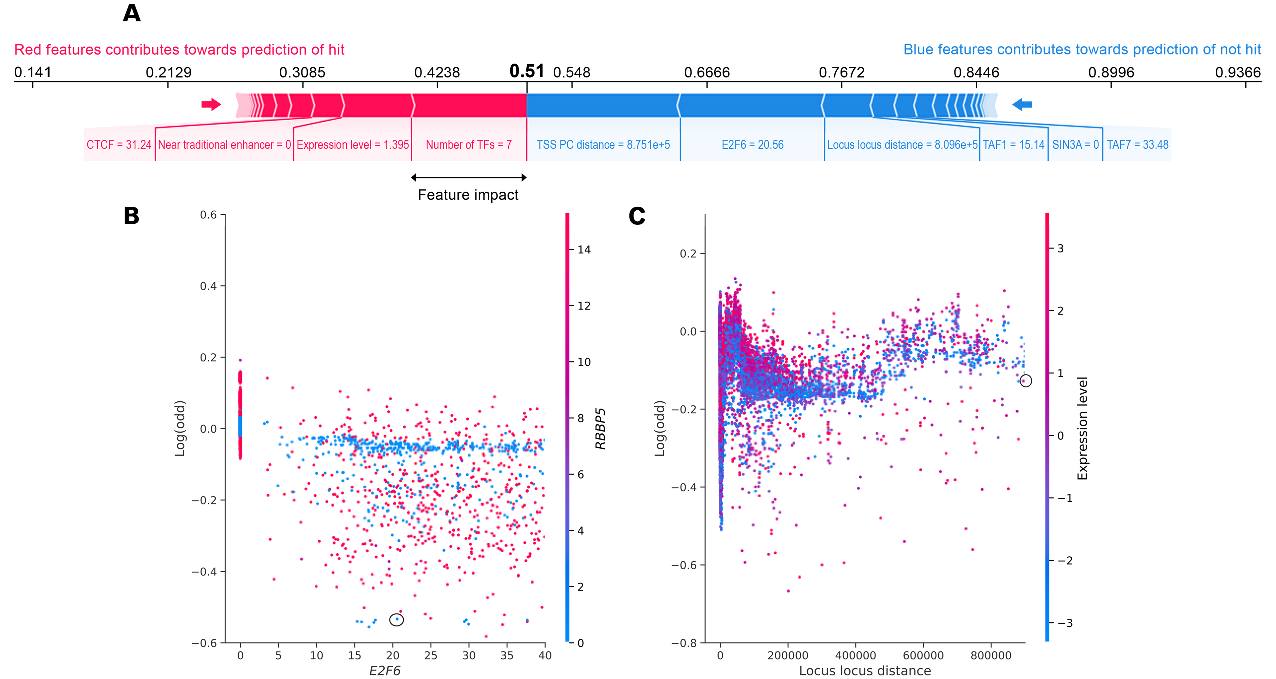
\includegraphics[scale=0.6]{plots/results/ml/model.exp.linc00798.pdf}
  \caption[Model explainability for \textit{LINC00879}]{\textbf{Model explainability for \textit{LINC00879}}. \textbf{(A)} Explained hit probability for \textit{LINC00879}. \textbf{(B)} SHAP dependence plots for \textit{E2F6}, and \textbf{(C)} lncRNA-PC distance distance versus their SHAP values. Circles highlight \textit{LINC00879}.}
  \label{fig:model-exp-lnc}
\end{figure}

The mild increased in hit probability shown in \autoref{fig:model-exp-lnc}A was driven mainly by 4 features: \textbf{1)} "\textit{number of TFs}", \textbf{2)} "\textit{expression level}", \textbf{3)} "\textit{distance from a traditional enhancer}", and \textbf{4)} \textit{CTCF}. The risk explanation bar in \autoref{fig:model-exp-lnc}A has red features that push the hit probabilities higher (to the right) and blue features that push the probabilities lower (to the left). Each group of features is sorted by the magnitude of their impact and the features with the greatest impact were labelled. Through this representation, we found that many of the 71 features had a small impact on \textit{LINC00879} case and the hit probabilities for \textit{LINC00879} were predominantly driven by 10 features. 

The reason \textit{LINC00879} obtained a 0.51 hit probability was mainly for being isolated from PCGs, the closest one being \textit{NSUN3}. This explains "\textit{TSS-PC}" and "\textit{lncRNA-PC distance}" features. Notably, transcription factors \textit{E2F6}, \textit{TAF1}, and \textit{TAF7} showed a negative effect. Next, to understand the role of these TFs SHAP dependence plots reported a correlation between \textit{E2F6} and \textit{RBBP5} (\autoref{fig:model-exp-lnc}B) , and "\textit{locus-locus distance}" and "\textit{expression}" (\autoref{fig:model-exp-lnc}C). For "\textit{locus-locus distance}" and "\textit{transcript expression}" two clusters were reveleaded, if "\textit{locus-locus distance}" increased on average the hit probability decreased unless transcripts presented an expression level > 0 FPKMs. For \textit{E2F6} and \textit{RBBP5} the clustering was less clear.  

\subsection{Further experimental validations to uncover cell-growth related lncRNAs}
\label{sec:list-lncRNA-validate}

The lncRNA \textit{LINC00879} was one example where our XGBoost model predicts a lncRNA transcript to be functional and the CRISRPRi library\autocite{liu_2017_crispri} labelled as not functional (false positive case). After thoughtful inspection of false positive transcripts in K562 cell, we selected a list of 40 transcripts to experimentally validate them (\autoref{tab:lncRNA-validate}), as we already validated \textit{LINC00879}.

Our aim is to uncover the maximum number of functional lncRNAs related to cell-growth, in the most efficient way, thus while we validate our candidate genes we could re-train our model. Following this approach, we could further understand the most important features that affect cell-growth and improve sensitivity and specificity values of our model. 

\begin{table}[!htb]
  \caption[List of 40 lncRNAs for experimental validation]{\textbf{List of 40 lncRNAs for experimental validation}}
  \begin{scriptsize}
    \begin{tabulary}{0.95\linewidth}{cccccc}
      \textit{AC005307} & \textit{AC005381} & \textit{AC010601} & \textit{AC012615} & \textit{AC074050} & \textit{AC096559} \\
      \textit{AC097532} & \textit{AC246817} & \textit{AL034397} & \textit{AL035446} & \textit{AL158066} & \textit{AL162413} \\
      \textit{AL691447} & \textit{AP000855}  & \textit{AP006222} & \textit{CUFF5183312} & \textit{FAM157C} & \textit{FAM41C} \\
      \textit{LINC00221} & \textit{LINC00680} & \textit{LINC00861} & \textit{LINC00879} & \textit{LINC01029} & \textit{LINC01203} \\
      \textit{LINC01410} & \textit{LINC01420} & \textit{LINC01608} & \textit{LINC02062} & \textit{LINC02154} & \textit{LINC02432} \\
      \textit{MINCR} & \textit{MIR4435-2HG} & \textit{NUTM2A-AS1} & \textit{NUTM2B-AS1} & \textit{PDXDC2P} & \textit{RP11-706O15} \\
      \textit{RP11-94P11} & \textit{SNHG1} & \textit{SNHG6} & \textit{ZFHX4-AS1} \\
    \end{tabulary}
  \end{scriptsize}
  \label{tab:lncRNA-validate}
\end{table}

\clearpage

\subsection{Discussion: XGBoost classifier to uncover the function of lncRNAs in cell-growth}
\label{sec:ml-discussion}

CRISPRi (CRISPR interference) is an established genome-wide technology to knockdown lncRNA transcripts in diverse cellular contexts. While the idea to inhibit lncRNA transcription in a high-throughput level is not novel,\autocite{liu_2020_crispri,Haswell_2021_crispri} the present work brings novelty in the field by combining: \textbf{1)} the supervised extreme gradient boosting (XGBoost) algorithm, \textbf{2)} transcription factor (TF) ChIP-seq data, and \textbf{3)} high-throughput screens to uncover the function of lncRNAs in the following human cell lines: iPSC, K562, U87, MCF7, MDA-MB-231, HeLa, and HEK293T. 

More importantly, our work added value by unveiling the cell-growth role of \textit{LINC00879} in the K562 cell line, with the aid of our cost-sensitive XGBoost classifier trained with Liu \textit{et al.} CRISPRi and ENCODE TF ChIP-seq datasets.\autocite{liu_2020_crispri,encode_2011_user,encode_2004} We were able to quantify the advantage of adding TF narrow-peaks around lncRNA core promoters, using XGBoost, and recursively eliminate non-contributing features based on Shapley values. We obtained a performance of mean AUROC of 0.8250 with our approach, which overperformed when compared to previous results (mean AUROC of 0.753\autocite{liu_2020_crispri}). Additionally, we obtained balanced sensitivity and specificity values (0.8227 and 0.7292, respectively) across all seven studied cells, even with a clearly under-representation of hits compared to not hits (on the order of 1:55). As a result of our satisfactory hit-classifier performance plus an association of the previously unknown \textit{LINC00879} with K562 cell-growth rate; 40 lncRNA genes with unknown function were selected as candidates for experimental validation in the K562 cell type. 

By obtaining the local and global explanations of our trained classifier with the 71 selected features (16 from the CRISPRi screening, and 55 from ENCODE TFs) based on Shapley values, our study showed that "\textit{distance between lncRNA-TSS and its nearby coding gene}", "\textit{expression level}", and "\textit{number of TFs with ChIP-seq signal}" features were the top 3 most important for our tree-based model. The feature "\textit{number of TFs}", to the best of our knowledge, is the first time that is highlighted to be relevant, using ML algorithms. In contrast, the importance of "\textit{expression level}" to link functionality to a noncoding locus, is a well-recognized result.\autocite{liu_2020_crispri,Haswell_2021_crispri} Moreover, Shapley values suggested that some genomic features, that globally may not be relevant, may actually be important for some specific transcripts. This suggests that lncRNAs involved in cell-growth follow a non-linear relationship with the described features, implying the necessity for functional screenings.

Nonetheless, CRISPRi  screens display non-negligible off-target effects. Additionally, a number of publications have reported that reverse-genetics assays show discrepancies among the cellular phenotypes and the number of differentiated genes obtained with different inhibition methods.\autocite{stojic_2018_specificity} More importantly, a very large gap exists between reporting biological function of lncRNAs in cell lines and the difficulty in obtaining such evidence in \textit{in-vivo} studies; this is true even for the lncRNAs considered as "\textit{gold standard}", such as \textit{Malat1}, \textit{Neat1}, etc.\autocite{gao_2020_reverse_genetics}  We obtained increased power to discriminate between hits and not hits by adding TF ChIP-seq data. This indicates that there is still room for improvement. For instance, conservation information (\textit{e.g.} sequence-conservation of promoters, transcripts and exon transcripts; plus synteny data) should be incorporated to understand how this feature plays a role to uncover noncoding transcripts involved in cell-growth; and adding more biological interpretability. Further, as distance between lncRNA TSS and its nearby protein-coding gene was ranked as the most important feature for our work, a more comprehensive lncRNA genomic-classification (\textit{i.e.} divergent lincRNA, convergent lincRNA, nested genic-exonic or intronic, etc.) should be included. Additionally, including splicing efficiency across ENCODE cell lines could be beneficial for our mode, as it has been for Haswell \textit{et al.}\autocite{Haswell_2021_crispri} Moreover, as the \textit{LINC00879 UCSC} plot reported, ENCODE epigenetic features should also be incorporated.  

In future implementations, our work could benefit from new available functional screenings based on CRISPRi and individual experimental validations from lncRNA candidate genes to re-train our model (\textit{e.g.} the results of our 40 lncRNA candidates); achieving a dynamic process. For instance, the new available CRISPRi library produced from Haswell \textit{et al.}\autocite{Haswell_2021_crispri} could be used as a validation-set for a robustness assessment of our algorithm; in addition to increasing the lncRNA hit percentage. This dynamic process could lead to the development of a web interface available to the community to serve as a predictive-tool to uncover functional lncRNAs in the context of cell-growth, and eventually other phenotypes, in human cell lines. All our analyses were based on supervised ML methods. However, we could harness the  weakly-unsupervised and the unsupervised strategies to allow the ML models to learn from the data itself. One analysis that can be performed is using the entire highly dimensional dataset and performing a k-means clustering; collapsing the data into two dimensions. Subsequently, visualizing the results through a t-SNE or UMAP plot. What we would expect to see is two different clusters, hits and not hits, nonetheless this result is unlikely because hit and not hits share a lot of common features, the latter result was observed by.\autocite{Haswell_2021_crispri}

At the early stage of our study, we tried to use the data from the \textit{LnCompare} database,\autocite{carlevaro_2019_lncompare} which contains interesting features full of biological richness, such as subcellular localization, expression across human tissues, tissue specificity (using the $\tau$ metric), etc. Nevertheless, the information is at the gene level instead of the transcript level, consequently we could not use that dataset. So collaborating with the \textit{LnCompare} developers to achieve transcript level data could be relevant for this project and for the lncRNA field.  

\clearpage

\section[LncRNA analysis of the \textit{Drosophila} genome during regeneration]{LncRNA analysis of the \textit{Drosophila} genome during regeneration}
\label{sec:results-dme}

\subsection{Characterization of cell-damage lncRNAs}
\label{sec:ge-reg-results}

To elucidate the role of lncRNAs within the \textit{Drosophila melanogaster} genome after cell-death induction, Vizcaya-Molina \textit{et al.}\autocite{vizcaya_2018} data was analyzed, using three time points after cell-damage: early (0h), mid (15), and late (25h). QC results demonstrated problems with replicate: \textit{control-0h-r2}, with a variability > 3 standard deviations from the rest of replicates (\autoref{supp-fig:connectivity-reg}) . In consequence, replicate \textit{control-0h-r2} was removed.

131 differentially expressed (DE) lncRNAs were identified. DE results revealed the early time point with the highest number of upregulated lncRNAs (\autoref{fig:dge-pc-lncRNA}A). Interestingly, downregulated lncRNAs at 15h obtained the highest number of DEGs, with 56 cases (see \autoref{tab:deg_complete}). As expected, lncRNAs demonstrated a time point specific expression, with 4 and 7 DEGs in all time points (\autoref{fig:dge-pc-lncRNA}B). 

\begin{figure}[!htb]
  \centering
  \includegraphics[scale=0.33]{plots/results/dme/PC.lncRNA.results.pdf}
  \caption[DE genes after cell-death induction]{\textbf{DE genes after cell-death induction}. \textbf{(A)} Number of lncRNA and PC DEGs. \textbf{(B)} LncRNA venn diagrams in early, mid, and late time-points. \textbf{(C)} PCG venn diagrams.}
  \label{fig:dge-pc-lncRNA}
\end{figure}

For PCGs, 1,627 DE genes were identified among them the \textit{reaper} (\textit{rpr}) and the \textit{Growth arrest and DNA damage-inducible 45} (\textit{Gadd45}) genes were found upregulated at 0h. \textit{Gadd45} is known to be required in response to stress, apoptosis, and proper regeneration of wing imaginal discs,\autocite{camilleri_2019,blanco_2010} and \textit{rpr} was the gene used to induce cell-damage.\autocite{vizcaya_2018} PCGs compared with lncRNAs showed a higher overlap of DEGs in the three time points (\autoref{fig:dge-pc-lncRNA}C).

LncRNA time-point and regeneration-specificity results revealed the early time-point with the highest number of genes experimenting with a time-point-specific expression with 14 and 8 genes expressed only at 0h or at 0h and 15h, respectively (\autoref{fig:time-point-reg-specific}A).  Same pattern was observed for regeneration specific expression (\autoref{fig:time-point-reg-specific}B). Increased time-point specificity at the early time point was preserved by dividing the genes by their DE status (\autoref{fig:time-point-specific-up-down}). 

\begin{figure}[ht!]
  \centering
  \includegraphics[scale=0.6]{plots/results/dme/time.point.reg.specificity.pdf}
  \caption[Time-point and regeneration-specificity results]{\textbf{Time-point and regeneration-specificity results}. \textbf{(A)} Time-point specificity analysis of the 131 DE lncRNAs. Time Point (TP) specific= lncRNA expressed only on the analyzed time-point. \textbf{(B)} Regeneration analysis of lncRNAs upregulated. Reg specific= not expressed in control.}
  \label{fig:time-point-reg-specific}
\end{figure}

We explored the DE status of the 131 DE lncRNAs across regeneration; identifying that 4 up and 7 down genes were DE in all time points, and that the vast majority of upregulated and downregulated genes were DE at the early time point and then not differentially expressed (NDE) in other time points (\autoref{fig:chracterization-lncRNAs}A). For lncRNAs NDE at 0h the majority were downregulated at 15h and then NDE at 25h. Two hairpin genes and \textit{CR40469} were the top 3 most expressed genes that were upregulated at 0h. Moreover, \textit{CR34335} and \textit{rox2} were the most expressed downregulated genes at 0h. To evaluate whether our differentially expressed lncRNAs were indeed not coding, coding potential assessment tool (CPAT) was used to score for coding potential.\autocite{wang_2013_cpat} Comparing the CPAT score of our DE lncRNAs to FlyBase annotated lncRNAs and PCGs expressed indicated that our DE lncRNAs reported a very low coding potential (\autoref{fig:chracterization-lncRNAs}B). None of our genes exceeded the threshold of 0.39, calibrated for discriminating coding from noncoding genes in \textit{Drosophila melanogaster} (\textit{D. melanogaster}).\autocite{wang_2013_cpat}

The 2,455 lncRNAs annotated within \textit{D. melanogaster} were dispersed throughout the genome, including intergenic (56.54\%), genic intronic (17.11\%) or genic exonic (26.35\%), with respect to neighboring PCGs (\autoref{fig:gw_lncRNA_class}).  In our DE set, intergenic was the most frequent class for early up with 44.83\% and for ealry down with 57.58\% (\autoref{fig:chracterization-lncRNAs}C); genome-wide intergenic lncRNAs were also the most common class. Interestingly, for upregulated genes at 15h genic intronic was the most frequent group (\autoref{supp-fig:mid-late-class}A; \textit{p-value}= 1.17e$^{-4}$; \textit{two-sided Fisher exact test}). On average, the percentage of overlapping between DE genic-exonic and their PCGs was 27.9\%, which was significantly lower than the rest of annotated genic-exonic genes (\textit{Wilcoxon test}, \textit{p-value}= 2.08e$^{-6}$).

\begin{figure}[ht!]
  \centering
  \includegraphics[scale=0.37]{plots/results/dme/chr.lncRNA.early.v2.pdf}
  \caption[LncRNA patterns after cell-damage]{\textbf{LncRNA patterns after cell-damage}. \textbf{(A)} Behavior of the 131 DE lncRNAs across regeneration. \textbf{(B)} Coding potential of the 131 DE lncRNAs, all annotated lncRNAs, and PCGs. \textbf{(C)} LncRNA classification of early DE lncRNAs. }
  \label{fig:chracterization-lncRNAs}
\end{figure}

Subclassification of lncRNAs highlighted divergent lincRNAs (long intervening noncoding RNAs) and intronic nested genes as the most representative subgroups of intergenic and intronic classes, respectively (\autoref{tab:lncRNAs-subclass}). Distance analysis between lncRNA TSS and PCG demonstrated that our DE subgroup of divergent lincRNAs (2,499 bp) presented a significantly lower distance compared to genome-wide divergent lincRNAs (4,153 bp; \textit{Wilcoxon test}, \textit{p-value}= 0.012), which may reflect a biological importance to be near from a PCG. Further, ATAC-seq results consistently with gene expression and DE analyses, indicated that in the early stage the TSS of upregulated lncRNAs were more accessible in regeneration compared to downregulated, and NDE lncRNA genes (\autoref{fig:atac-seq}). 

\begin{figure}[ht!]
  \centering
  \includegraphics[scale=0.7]{plots/results/dme/atac.seq.agg.early.pdf}
  \caption[ATAC-seq profiles for DE and NDE lncRNAs at the early time point]{\textbf{ATAC-seq profiles for DE and NDE lncRNAs at the early time point}. Aggregation plots around the TSS of up, down, and NDE lncRNAs ($\pm$400 bp) at the early stage of cell-death induction (0h). NDE= not differentially expressed lncRNAs.}
  \label{fig:atac-seq}
\end{figure}

\subsubsection{PCGs associated to the DE lncRNAs are enriched in cell-death and developmental terms}
\label{sec:go-lncRNAs}

Gene ontology (GO) enrichment of neighboring and overlapping PCGs (see \nameref{sec:gene_ontology_enrichment}) was used to assess the potential biological function of lncRNA genes within regeneration. After correction for multiple testing, overlapping PCGs showed significant GO terms for: programmed cell death, regulation of cell cycle and development (\autoref{fig:go_genic_intergenic}A). Subsequently, we combined neighboring and overlapping PCGs identifying more biological terms, such as: wing imaginal disc morphogenesis and development, \textit{Jak-STAT} cascade, and developmental processes (\autoref{fig:go_genic_intergenic}B). The \textit{Jak-STAT} pathway is required for regenerative growth and interestingly is not likely to occur in development, which may indicate that PCGs associated with the DE lncRNAs are involved in regeneration pathways and wound healing processes.\autocite{katsuyama_2015,santabarbara_2015}

\begin{figure}[ht!]
  \centering
  \includegraphics[scale=0.65]{plots/results/dme/go.genic.intergenic.pdf}
  \caption[GO terms of PCGs associated with the DE lncRNAs]{\textbf{GO terms of PCGs associated with the DE lncRNAs}. \textbf{(A)} GO of PCGs which overlapped a genic DEG. \textbf{(B)} GO based on the combination of PCGs which overlapped a genic DEG, and the two closer PCGs (up and down stream) from a lincRNA DEG. Size of circles denote number of genes of each term.}
  \label{fig:go_genic_intergenic}
\end{figure}

\subsubsection{Relationships between lncRNAs and nearby PCGs}
\label{sec:lncRNA-PC-correlation}

The relationship between lncRNAs and their neighboring PCGs during regeneration was assessed by following two approaches. First, by analyzing the DE status of each gene type (\nameref{paragraph:de-status}). Second, by classifying their expression pattern during wound healing (\nameref{paragraph:expression-classification}).

Each lncRNA was assigned to its overlapping or closest PGC (see \nameref{sec:lncRNA_pc_co-expression}), forming lncRNA-PCG pairs that were used to evaluate their association. We obtained 134 pairs for lincRNA-PCG, with a maximum of 1 lincRNA (\textit{CR42868}) neighboring 10 PCGs. On average, the divergent-lincRNA class was the closest subgroup to their neighboring PCGs (\autoref{supp-fig:lincRNA-distance}). Subsequently, we combined the 134 lincRNA-PCG pairs with 76 genic-PCG pairs obtaining a total of 210 lncRNA-PCG pairs. We allowed multiple-overlaps for genic lncRNAs; the genic-exonic \textit{CR45600} overlapped with 3 PCGs, which was the locus with the highest overlap number.

\paragraph{The DE status of lncRNA-PCG pairs reveal low relationship}
\label{paragraph:de-status}

Investigation of the DE status of lncRNA-PCG pairs demonstrated a low relationship between them. On average, 90\% of PCGs were flat while the lncRNAs were DE. At the early time point in regeneration, and at the mid time point in control were the highest and lowest percentages of relationship, respectively (\autoref{fig:co-exp-cat-2}A,B). Interestingly, \autoref{fig:co-exp-cat-2} reported more concordant cases in all our studied conditions.

\begin{figure}[ht!]
  \centering
  \includegraphics[scale=0.55]{plots/results/dme/co.expression.cat.pdf}
  \caption[DE status of PCGs nearby DE lncRNAs]{\textbf{DE status of PCGs nearby DE lncRNAs}. \textbf{(A,B)} In regeneration or in control, respectively.}
  \label{fig:co-exp-cat-2}
\end{figure}

At the early time point, 16\% relationship represented 8 concordant cases (5 genic-exonic, 2 genic-intronic and 1 intergenic) and 1 discordant case (1 intergenic). Additionally, 44\% of neighboring PCGs were uncharacterized, and characterized PCGs were involved in metabolic processes.

\begin{figure}[ht!]
  \centering
  \includegraphics[width=1\textwidth]{plots/appendix/dme/cr43611.ucsc.plot.pdf}
  \caption[\textit{CR43611 UCSC} plot]{\textbf{\textit{CR43611 UCSC} plot}. RNA-seq data, gene structure, conservation, and repeats of \textit{CR43611} lncRNA. Blue boxes represent coding and noncoding genes. .}
  \label{fig:cr43611-ucsc}
\end{figure}

An interesting concordant case was the \textit{CR3611}-\textit{chaski} (\textit{chk}) pair (genic-intronic and PCG, respectively) which both were upregulated at all time points (\autoref{fig:cr43611-ucsc}). The \textit{chk} gene has been observed to be involved under stress conditions in glial cells.\autocite{delgado_2018} For the discordant case, the intergenic \textit{CR44899} was only upregulated at the early time point and its neighboring PCG \textit{CG13258} was downregulated at the three time points (\autoref{supp-fig:cr43611-ucsc}). To the best of our knowledge, the role of \textit{CG13258} is unknown. These analyses allowed us to establish a relationship between \textit{CR3611} and \textit{CR44899} lncRNAs and their neighboring PCGs ("\textit{guilt-by-association}" \textit{in-cis}\autocite{signal_2016_computational}), although more analyses are needed to confirm their relationship. 

\paragraph{Classification of lncRNA-PCG expression show higher relationship}
\label{paragraph:expression-classification}

Using our expression classification approach (see \nameref{sec:lncRNA_pc_co-expression}) resulted in 33\% more lncRNA PCG relationships compared to observing the DE status of lncRNA PCG pairs. Focusing on regeneration, we identified that most of the DE lncRNAs were labeled as decreasing, followed by valley, peak and increasing classification (\autoref{fig:co-exp}A), in contrast peak and valley were the top 2 more common classes in control (\autoref{supp-fig:co-exp-ctrl}A).  

\begin{figure}[ht!]
  \centering
  \includegraphics[scale=0.6]{plots/results/dme/co.expression.results.pdf}
  \caption[Co-expression results]{\textbf{Co-expression results}. \textbf{(A)} Co-expression classification in regeneration. \textbf{(B)} Co-expression results in regeneration. \textbf{(C)} Summarization of different co-expression associations in control and in regeneration.}
  \label{fig:co-exp}
\end{figure}

On average, we identified 44\% of gene expression association between lncRNA-PCG pairs. As well as with our previous analysis, we found more concordant cases (36 cases for control and regeneration conditions; \autoref{fig:co-exp}B and \autoref{supp-fig:co-exp-ctrl}B). We observed a higher number of lncRNA-PCG associations using this approach compared to the former approach (observing the DE status of lncRNA-PCG pairs), the reason is this approach is less restrictive. 

Interestingly, by focusing in regeneration and by their genomic position, the relationship frequencies order changed, for genic-intronic the most common case was concordant instead of no association, suggesting a higher probability of \textit{cis-acting}  mechanism between genic intronic and their overlapping PCGs\autocite{perez_blister, pelechano_2013} (see \autoref{fig:co-exp-supp-fig}A). Peak and valley were the most common classes for concordant and discordant scenarios, respectively (\autoref{fig:co-exp-supp-fig}B). Combining regeneration and control relationship results demonstrated as expected no-association between lncRNA-PCG pairs as the most common case (\autoref{fig:co-exp}C). Additionally, a higher association in control compared to regeneration was reported. However, we were more interested in cases where we observed positive and negative associations both in control and in regeneration (\autoref{fig:co-exp}C). Hence, we thoroughly examined 15 and 10 positive and negative associations, respectively.

\begin{figure}[ht!]
  \centering
  \includegraphics[scale=0.6]{plots/results/dme/co.expression.examples.pdf}
  \caption[\textit{CR40469} and \textit{CR43956} co-expression]{\textbf{\textit{CR40469} and \textit{CR43956} co-expression}. \textbf{(A)} Concordant in control and discordant in regeneration. \textbf{(B)} Concordant in control and in regeneration. Expression= log$_{10}$(TPM+0.1).}
  \label{fig:co-exp-examples}
\end{figure}

\textit{CR40469}-\textit{RhoGAP1A} and \textit{CR43956}-\textit{anne} pairs were two examples of a positive-negative and a positive-positive association in control and in regeneration, respectively. The lincRNA \textit{CR40469} has a distance of 4.7 Kb from its neighbor PCG \textit{RhoGAP1A}, \textit{CR40469} was upregulated at 0h and 25h, and \textit{RhoGAP1A} was expressed but NDE in all time points. In control, the  \textit{CR40469}-\textit{RhoGAP1A} pair displayed the same expression pattern, with higher expression at the mid time point. By contrast, during regeneration \textit{CR40469} changed its expression from peak to valley (opposite expression pattern); and \textit{RhoGAP1A} maintained the same expression pattern (\autoref{fig:co-exp-examples}A). These results suggest a relationship between \textit{CR40469} and \textit{RhoGAP1A}, thus are an interesting pair to experimentally validate this initial hypothesis. 

The genic-intronic \textit{CR43956} overlaps in antisense with the PCG \textit{anne}, \textit{CR43956} was downregulated at 15h, and \textit{anne} was downregulated at 25h. The \textit{CR43956}-\textit{anne} pair demonstrated the same pattern of expression both in control and in regeneration (\autoref{fig:co-exp-examples}B). In consequence, there could be other interesting pairs to further analyze. 


\subsubsection{Functional and non-functional genomic features for our DE lncRNAs}
\label{sec:genomic-features}

DE lncRNAs presented an over-representation of genes with multiexons on their longest transcript compared to NDE (\textit{Fisher exact test}, \textit{p-value}= 0.0104; \autoref{supp-fig:number-exons}). According to Liu \textit{et al.} logistic regression model,\autocite{liu_2017_crispri} number of exons is a mild feature for lncRNA functionality (odds= 1.1 and \textit{p-value}= 5.74e$^{-3}$). Additionally, lncRNAs with multiple isoforms were more present in DE lncRNAs, compared to NDE (\textit{Fisher exact test}, \textit{p-value}= 4.36e$^{-5}$; \autoref{supp-fig:isoform-analysis}). 

Overall, lncRNA exons showed a lower GC content compared to PCG exons (\textit{Wilcoxon test}, \textit{p-value}= 1.56e$^{-7}$) as observed by.\autocite{lopez_2017} In addition, analyzing GC\% of promoters, genes, and the longest transcript from DE and NDE lncRNAs, significant lower GC content was observed with 0.0185, 1.09e$^{-6}$, and 2.44e$^{-5}$ adjusted \textit{p-values}, respectively (\textit{Wilcoxon test}; \autoref{supp-fig:gc-content}). Next to better understand GC content results, analyses based on lncRNA classification, and comparing DE to lncRNA expressed and not expressed (NE) were performed. We Iidentified significant differences among intergenic lncRNAs, with 0.01 and 6.01e$^{-4}$ adjusted \textit{p-values}, respectively (\textit{Wilcoxon test}; \autoref{fig:genomic-cha}A). High GC content has been observed in functional lncRNAs with more stable secondary structures,\autocite{lopez_2017} however GC\% is not the most determinant feature to assign functionality to lncRNAs.\autocite{haswell_2020}

Finally, length analyses based on the longest transcript reported a lower length contrasting DE genic intronic to NDE genic intronic (\textit{Wilcoxon test}, adjusted \textit{p-value}= 0.031; \autoref{fig:genomic-cha}B). 

\begin{figure}[ht!]
  \centering
  \includegraphics[scale=0.6]{plots/results/dme/gc.length.pdf}
  \caption[Genomic features of our lncRNA DE list]{\textbf{Genomic features of our lncRNA DE list}. \textbf{(A)} GC\% between DE, expressed, and NE. \textbf{(B)} Length analysis based on the longest transcript, \textit{y-axis} in log$_{10}$(bp). Expressed= lncRNA expressed in control or/and regeneration, NE= not expressed, and n.s.= not significant.}
  \label{fig:genomic-cha}
\end{figure}

\subsubsection{Low sequence-conservation for our DE lncRNAs in 27 insect species}
\label{sec:sequence-conservation}

Sequence-conservation was defined as homology higher than 0.25 in at least \textit{D.melanogaster} and other insect species (\autoref{fig:seq-conser-early}C).  Conservation analyses were performed at two levels: gene, and transcript with 35.88\%, and 59.54\% of lncRNAs conserved from the 131 group of DE genes, respectively. As expected, at transcript level lncRNAs were more conserved compared to gene level, where lncRNA introns are less conserved.\autocite{lopez_2017,nitsche_2017,ulitsky_2016_evolution}

No statistical difference was observed between DE and NDE genes. Moreover, by their location classification, the lincRNA (lincRNA and intergenic terms were used indistinctly) group was the most conserved at gene and transcript level, with 24 and 39 conserved lincRNAs, respectively. To observe in more detail the conservation of lncRNAs within their time point and DE status, we plotted each conserved lncRNA by early (\autoref{fig:seq-conser-early}A), mid (\autoref{supp-fig:lncRNA-seq-conservation}A), and late (\autoref{supp-fig:lncRNA-seq-conservation}B) time points.

At the early time point, 38.71\% and 61.29\% were conserved at gene and transcript level, respectively; from which 11 exonic, 6 intronic and 21 intergenic were conserved at the transcript level (\autoref{fig:seq-conser-early}A). \textit{CR45182} (4 species, 0.833 homology, and downregulated), \textit{CR44993} (24 species, 0.698 homology, and upregulated), and \textit{CR45433} (3 species, 1 homology, and upregulated) were the most conserved by exonic, intronic, and intergenic classification, respectively. Highlighting by DE status and lncRNA classification, genic-exonic up (58.33\%) and intergenic down (78.95\%) were the most conserved subgroups (\autoref{fig:seq-conser-early}B). Unclear sequence conservation clustering was observed between up and down genes, except for genic-intronic at the late time point (\autoref{supp-fig:lncRNA-seq-conservation}B).

\begin{figure}[ht!]
  \centering
  \includegraphics[scale=0.75]{plots/results/dme/seq.by.exon.pdf}
  \caption[Sequence-conservation of early DE lncRNAs at the transcript level]{\textbf{Sequence-conservation of early DE lncRNAs at the transcript level}. \textbf{(A)} Dots represent a lncRNA, and \textit{y-axis} reports the number of species that present the lncRNA conserved. \textbf{(B)}. Conserved and not conserved genes by DE status, and classification. \textbf{(C)} Phylogenetic tree with the 27 insect species used for the conservation analysis.}
  \label{fig:seq-conser-early}
\end{figure}

\clearpage

\subsection{LncRNA developmental and tissue signatures}
\label{sec:dme-results-second-part}

From the 131 DE lncRNAs in regeneration, we explored their general expression properties through development, using \textit{D. melanogaster} embryonic, larval, and pupal developmental stages obtained from the modENCODE project\autocite{celniker_2009,modencode_2010} (\autoref{fig:t-sne-mode-encode}A). Five well-known developmental PCGs were analyzed to assess a correct developmental pattern.\autocite{batut_2017} \autoref{supp-fig:markers-dev} confirmed an expected behavior from these five genes across embryonic development. The developmental markers \textit{Pgc}, \textit{Prd}, \textit{Gsb}, \textit{Mas} and \textit{Edg78E} showed an expression peak at 0-2h, 2-4h, 4-6h, 12-14h, and 18-20h, respectively. The same developmental oscillation was observed by Batut \textit{et al.}\autocite{batut_2017} In consequence, these results confirm the quality of the analyses and the developmental data.

\begin{figure}[ht!]
  \centering
  \includegraphics[scale=0.6]{plots/results/dme/modencode.fist.fig.pdf}
  \caption[t-SNE of developmental samples]{\textbf{t-SNE of developmental samples}. \textbf{(A)} Developmental time points analyzed. \textbf{(B)} t-SNE based on expressed genes, coding and noncoding, in log$_{10}$(TPM+0.1) within the developmental dataset.}
  \label{fig:t-sne-mode-encode}
\end{figure}

t-SNE based on expressed PCGs and lncRNAs revealed a clear cluster separation between embryonic and larval stages relative to pupal stages (\autoref{fig:t-sne-mode-encode}B), the same results were observed using a PCA (\autoref{supp-fig:pca-modencode}). Additionally, a timeline pattern and clustering among replicates were reported. 

Most of our DE lncRNAs in regeneration at the early time point showed dynamic expression patterns across development (\autoref{fig:heatmap-mod-dev}), 17.24\% and 24.24\% of lncRNAs upregulated and downregulated in regeneration, respectively were not expressed in the developmental time points used in our analysis. Hierarchical clustering of lncRNAs upregulated at the early time point highlighted 3 main clusters. In the first lncRNA cluster, genes were mainly expressed during embryonic time points (0h-24h). In the second cluster, genes were developmental-specific. Finally, the third cluster which represented the 8.3\% of lncRNAs, genes were highly expressed in all developmental time points (\autoref{fig:heatmap-mod-dev})

\begin{figure}[ht!]
  \centering
  \includegraphics[scale=0.6]{plots/results/dme/two.heatmaps.modencode.pdf}
  \caption[DE lncRNAs expressed through development]{\textbf{DE lncRNAs in cell-death conditions expressed through \textit{D. melanogaster} development}. Heatmaps based on gene expression (log$_{10}$ transformation plus 0.1 as a pseudo-count) of lncRNAs up and downregulated in regeneration (left and right plot, respectively). Developmental samples were collapsed by their mean expression and ascendingly sorted.}
  \label{fig:heatmap-mod-dev}
\end{figure}

Interestingly, the top 2 most expressed DE lncRNAs in regeneration were: \textit{hpRNA:CR33940} and \textit{hpRNA:CR32207}, which were also the top 2 most expressed in development from the 131 DE group. Similarly, \textit{CR34335}, \textit{rox2}, and \textit{CR43264} downregulated lncRNAs in regeneration were also the top 3 most expressed across development from the DE group. High gene expression of \textit{hpRNA:CR32207}, \textit{hpRNA:CR33940}, and \textit{rox2} within the regeneration and the developmental datasets can be linked to their stem-loop structure. LncRNA hairpin structures are linked to post-translational modifications and elevated gene expression,\autocite{statello_2021_lncRNA_reg} and lncRNA \textit{rox2} is part of the male-specific lethal complex (MSL) which is a key player in fruit fly dosage compensation.\autocite{flintoft_2013_rox,ilik_2013_rox} Single-cell analyses from Davie \textit{et al.} in \textit{Drosophila} brain highlight the lncRNA \textit{CR34335} as the few genes with no signals of decline with age and high mean expression,\autocite{davie_2018} these results are in agreement with our observations. 

Summarizing the three time-points analyzed in regeneration (early, mid and late), 24.76\% from the 131 DE lncRNAs were not expressed in the selected developmental samples, and 78\% of the DE genes in regeneration demonstrated condition-specific expression patterns. At the genome-wide level, 55.32\% of annotated lncRNAs were not expressed in any analyzed developmental stage, with the exception of 4\% of lncRNAs and the pupal stage, lncRNA presented condition-specific expression patterns (\autoref{fig:heatmap-modencode-dev-all}). Higher expression for lncRNAs in the pupal stage compared to embryonic and larval stages was also observed by.\autocite{chen_2016_lncRNA}

\subsubsection{DE lncRNAs present dynamic expression across development}
\label{paragraph:modENCODE-clusters}

K-means clustering was applied to more formally assess the dynamic expression of the DE lncRNAs in regeneration during development. According to the results from \autoref{fig:t-sne-mode-encode}B and \autoref{supp-fig:pca-modencode}, the clustering-analysis was applied dividing the developmental dataset in two groups: \textbf{1)} the embryo-larvae group and  \textbf{2)} the pupae group.

\begin{figure}[ht!]
  \centering
  \includegraphics[scale=0.6]{plots/results/dme/embryo.clusters.pdf}
  \caption[Six embryonic and pupal developmental clusters]{\textbf{Six embryonic and pupal developmental clusters}. K-means clustering based on embryonic and pupal gene-expression (blue and brown lines, respectively). \textit{Y-axis} shows the normalized and scaled gene-expression levels. \textit{X-axis} denotes the developmental time-points ascendingly sorted. Left-numbers show the number of the 131 DE lncRNAs contained in each developmental cluster.}
  \label{fig:k-means}
\end{figure}

Six clusters were obtained from the embryo-larvae group, containing 30 of the 131 DE lncRNA genes, with highly correlated expression during development (\autoref{fig:k-means}; mean \textit{Pearson's correlation}= 0.87). All embryonic-larval clusters contained lncRNAs DE in regeneration, the frequency of the DE lncRNAs within the clusters was balanced, although cluster 3 and cluster 5 contained the highest number of the DE lncRNAs with 6 genes in both clusters. Cluster 3 contained lncRNAs lowly expressed across all time points, and cluster 5 contained genes with a decreased expression trend and after embryo 22-24h an increase was observed. 

The larvae-group revealed nine robust-clusters, containing 49 of the 131 DE lncRNA genes, from which clusters 4, 5, 7, 8, and 9 (\autoref{fig:k-means-pupae}) presented more dynamics compared to clusters 1, 2, 3, and 6 (\autoref{supp-fig:pupae-clustering}), which were clustered for their expression level. The nine pupal-clusters contained at least one DE lncRNA; cluster 2 and cluster 4 contained the highest number of DE lncRNAs, with 14 and 8, respectively. In cluster 2, lncRNAs presented a mild decrease of expression during pupal development, and cluster 4 contained genes that decreased their expression from pupae 24h. 

\begin{figure}[ht!]
  \centering
  \includegraphics[scale=0.6]{plots/results/dme/pupae.clusters.pdf}
  \caption[Pupal developmental clusters]{\textbf{Pupal developmental clusters}. K-means clustering based on pupal developmental expression (green line). \textit{Y-axis} shows the normalized and scaled gene expression levels. \textit{X-axis} denotes the developmental time-points ascendingly sorted. Left-numbers show the number of the 131 DE lncRNAs contained in each cluster.}
  \label{fig:k-means-pupae}
\end{figure}

Clustering analyses of embryonic-larval and pupal groups highlighted the dynamic expression of the DE lncRNAs across development. Any over-representation was observed from our group of DE lncRNAs within a specific embryonic-larval cluster. In contrast, pupal clusters 9, 8, and 7 presented an under-representation of DE lncRNAs suggesting, on average, a steady and higher expression levels relative to the embryonic-larval group. 

\subsubsection{LncRNA tissue-specific expression patterns}
\label{sec:erc}

An imaginal-disc analysis was performed to observe the expression patterns of our 131 DE lncRNAs. \textit{D. melanogaster} antenna, eye, leg and wing imaginal discs RNA-seq data at three developmental time points\autocite{perez_blister} (L3, WPP and late pupae) was used (\autoref{fig:erc-tsne}A).

t-SNE results based on expressed genes (coding and noncoding) reported that the developmental time points were the most important factor for sample clustering (\autoref{fig:erc-tsne}B); the same pattern was observed using a PCA analysis (\autoref{supp-fig:pca-erc}). Differences between larval and pupal developmental time-points are in agreement with our prior developmental results (see \autoref{fig:t-sne-mode-encode}). Moreover, we visualized a clustering between antenna and eye imaginal disc samples in the three time points; these results are expected as antenna and eye imaginal discs come from the eye-antenna imaginal disc.\autocite{aldaz_2010_imaginal,spratford_2014_dissection} Thus, our exploratory results are in agreement with the literature. 

\begin{figure}[ht!]
  \centering
  \includegraphics[scale=0.6]{plots/results/dme/erc.scheme.t.sne.pdf}
  \caption[Imaginal disc data]{\textbf{Imaginal disc data}. \textbf{(A)} Retrieved imaginal discs at L3, WPP, and late pupae developmental time points. Scheme inspired by.\autocite{perez_blister} \textbf{(B)} t-SNE based on expressed genes in log$_{10}$(TPM+0.1) within the antenna, eye, leg, and wing imaginal disc data.}
  \label{fig:erc-tsne}
\end{figure}

110 of the 131 DE lncRNA genes were expressed at least in one imaginal disc. Focusing in the early time point after cell-death induction, 79.31\% and 78.79\% of lnRNAs upregulated and downregulated in regeneration were expressed within the imaginal disc data, respectively. Hierarchical clustering based on expression levels of genes upregulated at the early time point reported 4 clusters (\autoref{fig:erc-data}). Interestingly, the last two clusters presented a tissue and/or time point specific expression; and genes were on average only expressed at L3 and WPP or at late pupae time points, respectively. The lncRNA \textit{CR40469} showed the highest expression level at L3 time point in wing imaginal disc. Moreover, \textit{CR40469} was within a tissue and time-point specific-cluster.

On average, 38\% of lncRNAs upregulated were expressed in all imaginal discs and time-points without showing a specific pattern. Additionally, hairpin genes were highly expressed, except on the late pupae time point, where their expression decreased compared to the L3 and the WPP time points.

Within the imaginal-disc dataset expressed downregulated genes presented a higher expression level relative to upregulated lncRNAs (\autoref{fig:erc-data}), the same behaviour was observed within the developmental dataset. In addition, 24.2\% and 33.3\% of downregulated genes were highly expressed, and demonstrated tissue and/or time-point specific-expression patterns, respectively. Surprisingly, \textit{CR34335} at L3 in wing imaginal disc revealed its lowest expression compared to other imaginal discs and developmental stages.  

\begin{figure}[ht!]
  \centering
  \includegraphics[scale=0.6]{plots/results/dme/two.heatmaps.erc.pdf}
  \caption[Imaginal disc profiles of the DE lncRNAs in regeneration]{\textbf{Imaginal disc profiles of the DE lncRNAs in regeneration}. Expression heatmaps from lncRNAs upregulated and downregulated in the early time point of regeneration (left and right plot, respectively) in each imaginal disc and sorted from larval to late pupal developmental stages.}
  \label{fig:erc-data}
\end{figure}

At the genome-wide level, lncRNAs reported low expression within the imaginal disc dataset with 24\% of the 2,455 annotated lncRNAs expressed in at least one imaginal disc at any time point (\autoref{fig:heatmap-erc-all}). Higher gene expression was observed at the latest time point, these results are in line with.\autocite{chen_2016_lncRNA}

\clearpage

\subsection{Assessing the lncRNA:\textit{CR40469} function during \textit{D. melanogaster} imaginal-disc regeneration process}
\label{sec:results-cr40469}

To uncover the function of lncRNAs during regeneration, we selected the lncRNA \textit{CR40469} for targeted deletion using ends-out homologous recombination.\autocite{baena_2013} \textit{CR40469} was selected for KO for its increased expression after cell-damage at the early time point, where it was upregulated. Moreover, it was the top 3 most expressed noncoding locus from our DE list. Finally, \textit{CR40469} is an intergenic lncRNA isolated from coding genes. In consequence, its transcriptional inhibition could be more easily associated with \textit{CR40469} role instead of a characterized coding gene. Our target locus is located at the beginning of the X chromosome; the PCG \textit{CG17636} is \textit{CR40469} closest coding neighbor with a locus-locus distance of $\sim$1.7 Kb.  

\textit{CR40469} was homozygously knocked-out, next its transcriptome was sequenced in control and in regeneration conditions only at 0h after genetically inducing cell-damage. In addition, the \textit{CR40469} locus without genetic perturbation (\textit{CR40469}$^{Wt}$) was also sequenced in control and regeneration conditions at the early time point, to serve as a basis of comparison. Hence, we obtained 4 combinations: \textbf{1)} \textit{CR40469}$^{KO}$ in control at 0h, \textbf{2)} \textit{CR40469}$^{KO}$ in regeneration at 0h, \textbf{3)} \textit{CR40469}$^{Wt}$ in control at 0h and \textbf{4)} \textit{CR40469}$^{Wt}$ in regeneration at 0h (see \autoref{fig:cr40469-results}).


\begin{figure}[!htb]
  \centering
  \includegraphics[width=0.65\textwidth]{img/results/dme/CR40469-KO-results.png}
  \caption[\textit{CR40469} KO dataset]{\textbf{\textit{CR40469} KO dataset}. RNA-seq samples produced to study the role of \textit{CR40469} during imaginal disc regeneration.}
  \label{fig:cr40469-results}
\end{figure}

We obtained a high correlation among the RNA-seq replicates (mean Pearson correlation= 0.951; see \autoref{supp-fig:wgcna-cr40469} and \autoref{fig:qc-cr404-rna-seq}), and a high percentage of mapped reads (on average 98.32\%; see \autoref{supp-tab:cr40469-num-reads}). 

\subsubsection{Perturbation of \textit{CR40469} during regeneration display significant transcriptomic alterations}
\label{sub-sub-sec:cr40469-de-results}

534, 95, 159, and 255 differentially expressed coding and long noncoding genes were identified for the following comparisons: \textit{CR40469}$^{KO}$ vs. \textit{CR40469}$^{Wt}$ in control, \textit{CR40469}$^{KO}$ vs. \textit{CR40469}$^{Wt}$ in regeneration, regeneration vs. control with \textit{CR40469}$^{KO}$, and regeneration vs. control with \textit{CR40469}$^{Wt}$, respectively (\autoref{fig:cr40469-volcano-plots}). Upregulated genes were the most abundant class in the 4 comparisons, this proportion was maintained by inspecting by gene-biotype. Except for \textit{CR40469}$^{KO}$ vs. \textit{CR40469}$^{Wt}$ in regeneration, where downregulated genes were more present for lncRNAs (\autoref{supp-tab:cr40-ko-de}). \textit{Cacophony} (\textit{cac}), lncRNA \textit{CR44042}, and \textit{CG6701} were the only common DE genes in the 4 comparisons (the first two genes were up, and the last one was downregulated). 

\begin{figure}[ht!]
  \centering
  \includegraphics[scale=0.65]{plots/results/dme/condition.2.volcano.heatmap.pdf}
    \caption[DE results for \textit{CR40469}-KO vs. \textit{CR40469}-Wt in regeneration]{\textbf{DE results for \textit{CR40469}$^{KO}$ vs. \textit{CR40469}$^{Wt}$ in regeneration}. \textbf{(A)} DE between \textit{CR40469}$^{KO}$ and \textit{CR40469}$^{Wt}$ both in regeneration at 0h. \textit{Y-axis} displays significance for the comparison. Left and right numbers show down and up genes, respectively. \textbf{(B)} Top 15 upregulated coding and noncoding genes, based on their log$_2$ fold change. Columns represent the KO and Wt replicates, after cell-damage at 0h.}
  \label{fig:cr40469-de-volcano-2}
\end{figure}

The fourth comparison, which is comparing the expression profile between control and regeneration conditions without affecting \textit{CR40469} acted as a comparison framework (\autoref{fig:cr40469-volcano-plots}D). As expected, the \textit{rpr} pro-apoptotic gene (responsible for genetically induced cell-damage) was upregulated. Additionally, the \textit{Gadd45}, \textit{unpaired 3} (\textit{upd3}), \textit{moladietz} (\textit{mol}), and the \textit{LaminC} (\textit{LamC}) PCGs were upregulated; these genes were identified and validated in previous studies of wing disc regeneration.\autocite{vizcaya_2018, khan_2017_dme} On average, we observed $\sim$22\% of overlap between our comparison framework and previous reported results.\autocite{vizcaya_2018} This could be explained by different sequencing chemistry, number of replicates, sequencing depth, and DE methods.

Next, we are going to focus on the second comparison, where we assess the \textit{CR40469} role in regeneration (\textit{CR40469}$^{KO}$ vs. \textit{CR40469}$^{Wt}$ in regeneration). Deletion of the \textit{CR40469} locus caused significant changes in gene expression, compared with previous reported results for fruit fly lncRNA KO.\autocite{schor_2018} \textit{CR40469} significantly affected the expression of 95 genes (75 coding and 20 lncRNAs with an adjusted \textit{p-value} < 0.05), and obtained a median fold change of $\sim$1.41. Forty-eight of these were overexpressed in the KO line, and the remaining 47 genes showed decreased expression levels (\autoref{fig:cr40469-de-volcano-2}A and \autoref{supp-tab:cr40-ko-de}). GO results reported an enrichment for developmental pathways, which include the \textit{t} coding gene (\autoref{fig:cr40469-de-volcano-2}B).  

More importantly, after deleting \textit{CR40469} after inducing cell-death we observed a decreased wing area and aberrant pattering from wings (data not shown). These observations in addition to significant changes in gene expression suggest a role for \textit{CR40469} in wing discs during regeneration. 

\clearpage

\subsubsection{\textit{CR40469} shows a \textit{trans-acting} mechanisms within the X chromosome}
\label{sub-sub-sec:cis-acting}

After analyzing the global and local effects caused by \textit{CR40469} deletion, we identified an over-representation of DE genes across the X chromosome (\textit{Fisher exact test}, \textit{p-value}= 1.02e$^{-4}$), where our targeted locus is annotated (\autoref{fig:cr40469-cis-acting}A and \autoref{fig:cr40469-cis-acting}B). This over-representation was specific for \textit{CR40469}$^{KO}$ in regeneration; the rest of the comparisons reported an even distribution across \textit{Drosophila} chromosomes (\autoref{supp-fig:cr40469-cis-acting}). Further, non-significant genes were disrupted around $\sim$550 Kb, the closest one was the PCG \textit{CG42259}, which is 554 Kb away from the knocked-out gene. Interestingly, \textit{CG42259} is involved in response to wounding.\autocite{tattikota_2020_CG42259}

These preliminary results suggest \textit{CR40469} could act as a \textit{trans-acting} lncRNA on the X chromosome. Although, further analyses are required to confirm a modulation between the knocked-out locus and \textit{CG42259}, or other loci DE located on the X chromosome. 

\begin{figure}[ht!]
  \centering
  \includegraphics[scale=0.6]{plots/results/dme/cis.acting.pdf}
    \caption[\textit{CR40469} \textit{cis-acting} assessment]{\textbf{\textit{CR40469} \textit{cis-acting} assessment}. \textbf{(A)} Local impact of \textit{CR40469}$^{KO}$ on genes in proximity. \textbf{(Aa)} Across the X chromosome and \textbf{(Ab)} between the closest DE gene (\textit{CG42259}) and \textit{CR40469} locus. \textit{X-axis}= chromosomal distance; \textit{y-axis}= log$_2$ fold change. Only DE and expressed genes were plotted. \textbf{(B)} \textit{X-axis} shows the fruit fly chromosomes, where DEGs were observed. Percentage was calculated based on the number of DEGs by each chromosome divided by the number of expressed genes.}
  \label{fig:cr40469-cis-acting}
\end{figure}

\clearpage

\subsection{Discussion: LncRNA analysis of the \textit{Drosophila} genome during regeneration}
\label{sec:dme-discussion}

Our work brings novelty to the literature by studying the role of long noncoding RNAs (lncRNAs) in \textit{Drosophila} imaginal disc regeneration process, which even presenting an elevated homology to human biological processes and displaying elevated regeneration capacities,\autocite{vizcaya_2020_chromatin,ji_2019_understanding} the systematic study of lncRNAs in this regeneration model is poorly explored. We identified 131 differentially expressed (DE) lncRNAs comparing regeneration and control conditions from a public available RNA-seq dataset, using 3 time points (early: 0h, mid: 15h, and late: 25h time points after inducing cell-damage). Our results are in agreement with the lncRNA field, observing time-point and condition specific-expression. Moreover, we observed that the early time point showed the highest number of upregulated noncoding genes (29 lncRNAs), and an increased number of time-point and regeneration-specific genes (22 and 13 lncRNAs, respectively). Additionally, our DE lncRNAs demonstrated an over-representation of genes with multiple exons and isoforms compared to expressed and not differentially expressed (NDE) genes (0.0104 and 4.36e$^{-5}$ \textit{p-values}, respectively). Next, GC\% content and sequence-conservation in 27 insect-species was analyzed, comparing our 131 DE lncRNAs to expressed and NDE lncRNAs. For GC\%, we observed a significantly lower content (\textit{p-value}= 6.01e$^{-4}$), where higher GC\% is associated with functional genes.\autocite{liu_2017_crispri} Notably, we reported a non-association between DE-status and sequence-conservation; this contradictory mixture of functional (multiple number of exons and isoforms) and non-functional (GC\% and sequence-conservation) genomic features observed in our DE list, highlights the importance of reverse-genetic assays (\textit{e.g.} knockout and knockdown) to uncover lncRNA functionality.

After conducting an analysis observing the DE status of lncRNA-PCG pairs, we observed a low rate of relationship among them. However the \textit{CR3611}-\textit{chk} pair, (lncRNA and PCG, respectively) both were upregulated in the three analyzed time points, and could be an interesting pair to further study; assessing a possible "\textit{cis-regulatory effect}" of \textit{CR3611} on \textit{chk}, which is involved in stress conditions.\autocite{delgado_2018} We investigated the gene-expression behaviour of our 131 DE lncRNAs in developmental (from embryo to late pupae) and imaginal discs (antenna, eye, leg and wing imaginal discs) datasets, where we observed that $\sim$51.5\% were only expressed in cell-death conditions. Although, this result could also be linked with non-biological conditions, such as the available and the selected developmental time-points used in our study. On average, 91.7\% of the DE lncRNAs in regeneration which were expressed in the developmental or in the imaginal-discs datasets displayed a time-point expression pattern. This highly temporally restricted expression of lncRNAs during \textit{Drosophila} development was also observed by Chen \textit{et al.}, where as well as our study they reported the late embryonic and larval stages with higher lncRNA expression, reflecting the regulatory role of lncRNAs for the onset of metamorphosis.\autocite{chen_2016_lncRNA}

The lncRNA \textit{CR40469} was selected for a knockout experiment, as a consequence of our previous analyses within the regeneration dataset. The \textit{CR40469} genetic deletion showed significant transcriptomic alterations; we identified 95 genes with modified expression, when we compared \textit{CR40469}$^{KO}$ vs. \textit{CR40469}$^{Wt}$ in regeneration conditions at the early time-point. In addition, after studying the percentage of differentially expressed genes (DEGs) with expressed-genes by each fruit fly chromosome, we noticed an enrichment of DEGs in the X chromosome (\textit{p-value}= 1.02e$^{-4}$), where \textit{CR40469} is located. We hypothesize that \textit{CR40469} could act \textit{in trans}, affecting the expression of genes in the X chromosome, however further experiments need to be performed to confirm this. Interestingly, these findings based on genetic knockout are in contrast to previous publications on observing significant transcriptomics alterations. For instance, Shor \textit{et al.} after conducting an analysis based on RNA-seq data and CAGE data during fruit fly embryogenesis, they selected and knocked-out 2 lncRNAs, finding modest changes in expression (19 and 40 genes).\autocite{schor_2018} Moreover, one locus analyzed by the team was located in a gene-poor region, which the team suggested this lncRNA could act \textit{in trans}. Similarly, the lncRNA \textit{CR40469} is located in a gene-poor region (at the beginning of the X chromosome) and we suggested a similar mechanism for \textit{CR40469} during regeneration, in consequence our hypothesis to suggest a lncRNA mechanism is in agreement with prior studies.

In terms of limitations, although \textit{CR40469} was not conserved at the sequence-level using 27 insect-species, further conservation analyses are needed, such as a positional-conservation analysis, which have been reported could detect a higher rate of conserved genes,\autocite{ulitsky_2016_evolution} even between distant related species. Other limitation our work possesses is its number of mapped reads (on average $\sim$46 million reads), which is enough to explore annotated genes and perform differential expression analyses.\autocite{sims_2014_sequencing} However, it is not deep enough to uncover "\textit{novel lncRNAs}" or to explore the regeneration profile at the transcript-level (it is required > 100 million reads\autocite{zhao_2011_optimizing}), which could be interesting to study. Nowadays, there is an increasing number of pipelines to unveil "\textit{novel lncRNAs}". For instance, the \textit{lncEvo} pipeline\autocite{bryzghalov_2021_lncevo} allows to automatically identify "\textit{novel lncRNAs}" following an "\textit{align-then-assembly}" strategy (using \textit{Stringtie}), and its tailor for High-Performance-Computing (HPC) environments using Docker containers to allow reproducibility. Although, CAGE data is not available for cell-death conditions in \textit{Drosophila} wing imaginal disc, there is CAGE data available during fruit fly embryogenesis,\autocite{schor_2018} which could shed some light for our lncRNA-TSS. However, these findings should be considered with caution, as lncRNA transcription is a condition-specific event. Moreover, our genetic-deletion presented the limitation to be non-specific for \textit{CR40469}, this could lead to disruption of an undetected regulatory element (\textit{e.g.} enhancer or promoter), although H3K4me1 ChIP-seq signals in cell-death conditions were not detected.  Additionally, there have been reported discrepancies between the number of DEGs based on the knockout technology (\textit{e.g.} CRISPRi, RNAi, and AOs); in consequence confirmation with other knockout technology could add more strength to our findings. 

For future steps, a 3C-analysis could add meaningful information to confirm an interaction between \textit{CR40469} with nearby DEGs, such as the following genes: \textit{CG42259}, \textit{png}, and \textit{CG4313}, which are the top 3 closest DEGs nearby \textit{CR40469}. With these results, we can even start to hypothesize a mechanism of action for \textit{CR40469} during regeneration in \textit{Drosophila} imaginal disc. Additionally, sharing our RNA-seq data could be beneficial to the community; by using our transcriptome profile as a comparison frame-work for future investigations, the same applies to our code/bioinformatic-pipeline, which could be implemented in similar biological contexts. Our study could also be benefited with Fluorescent \textit{in situ} hybridization (FISH) images of the lncRNA \textit{CR40469} during regeneration (for the experimental condition without deleting \textit{CR40469}) to explore its cellular location during cell-death. As the lncRNA role in \textit{Drosophila} imaginal disc during regeneration is poorly explored and understood, generate a deep long-reads RNA-seq library, with rRNA-depletion instead of polyA as selection methodology (to capture lncRNAs without polyA), with more time-points after inducing cell-death, and regeneration CAGE data could be a very powerful tool to explore "\textit{novel lncRNAs}"  in the process of regeneration. With a list of annotated and \textit{novel} DE lncRNAs in regeneration, we could take advantage of \textit{Drosophila} features, including a life cycle well-studied, complex and well-characterized morphology and abundant gene editing tools (\textit{e.g.} CRISPRi, CRISPRa, CRISPR-Cas9) to conduct phenotypic experiments for the selected lncRNAs. 


